\section{Physics of Dust Devils}
\label{sec:physics}

%% \begin{itemize}
%% \item \st{phenomenological description}
%% \item \st{regions/frequency of occurance}
%% \item \st{review of sinclair, kanak and renno and other pertinent literature}
%% \item \st{known physics of dust devils and other cyclonic structures}
%% \item \st{dust-devil/tornado/hurricane genesis}
%% \item \st{scaling discussion as estimate of energy}
%% \item \st{dust-Devil Generation Concept}
%% \item \st{motivation of computational modeling{
%% \item draw regions
%% %\item eyewall
%% \end{itemize}

To motivate how best to \textit{engineer} a synthetic
dust devil, we first address what is known about the naturally occuring
phenomena. We therefore begin this section with a qualitative discussion
of dust-devils, followed by a review of the known physics and pertinent 
literature review. We then briefly outline how we intend to leverage
these physical processes as a method of usable energy generation. 


\subsection{Phenomenological Character of Dust Devils}

%\begin{itemize}
%\item chart from sinclair of frequency (they are driven by delta t)
%\item turning direction independent
%\item characteristic velocities and sizes
  %\item genesis diagram (thermal plume) -- mention ambient angular
  %vorticity 
%\item structure diagram and description
%\end{itemize}

No rigorous definition of a dust devil exists. This cannot be attributed
to the rarity of the process. Rather, the phenomena of dust devils are
remarkably ubiquitous. These whirlwinds have been
observed across a wide variety of terrains, climates and even on several
other planets\cite{Sinclair1969,Bluestein2004,JGR:JGR13978,JGRE:JGRE1660}. 
While it is difficult to pin down a precise definition, several features 
are characteristic of a dust devil. They are regions of
intense vorticity and rotation, coupled with strong upward motions 
that are strong enough draw and lift particles along with the flow.
They are a self-sustaining vortex that maintains a funnel-like
chimney driven by hot air moving both upward and circularly. 
While they typically exist for only a few minutes, some have 
been observed to exist for significantly longer. While the velocities are 
typically several meters per second, 
%
% stolen from: http://glossary.ametsoc.org/wiki/Fujita_scale
%
dust devils occasionally are strong enough to cause damage and injury,
with some reaching F1 on the Fujita Tornado intensity
scale\cite{Edwards_tornadointensity}, with velocities between 33 and 49
$m/s$. 
%
% F1 (moderate damage): 33-49 m s-1
%
% ``F1 - Surface of roofs peeled off; mobile homes pushed off foundations
% or overturned; moving autos pushed off road. ``
Diameters range from about one meter to greater than thirty.  Their
average height is about thirty meters, but a few have been observed 
as high as 1 km or more. There appears to be no preferred direction, and
they are observed to rotate anticyclonically as well as
cyclonically. Although the vertical velocity 
is predominantly upward, the flow along the a central axis of large dust
devils may be downward. 
%
% cite martian dust devils
%
%Moreover, actual dust devils have been photographed from orbit, with
%some of them as large as 1 to 2 kilometers across at their base and 10
%km tall. 
Similarly visibly structured phenomena have been spotted over water, in
intense forest fires, or even in cold or freezing environments. 
%
% good place to ref jacobson2005fundamentals
%
This is to say nothing of other similar cyclonic phenomena, such as
tornados and hurricanes. 

While the phenomena is pervasive, certain 
environmental conditions do impact the frequency of formation
of dust devils. Sinclair\cite{Sinclair1969} provides perhaps the most 
systematic investigation characterizing favorable conditions for
formation. From these results we conclude that dust devils are most
likely to form at solar noon, the time of the greatest incident radiation 
on the ground. Furthermore, they are more likely to form in locations 
with a higher surface temperature. Moderate to high wind speeds (2-5
m/s) encourage dust devil genesis, but greater velocities (11 m/s)
appear to impede formation. They are more likely to be observed in
relatively flat locations, such as deserts.  

While there are existing publications on the numerical simulation of dust
devils, they are typically LES simulations that point
towards the occurance of similar phenomena within existing climate and
atmospheric models\cite{QJ:QJ200513160722,doi:10.3137/ao.420105}. Actual
measurements made inside a dust devil 
are limited. The available data hints that dust devils can be broken
into two regions: a low surface layer and a higher invisid region. The
low surface region is the  principle location of radial inflow. 
It is at the top of this region that the flow 
reaches its peak velocity, with that peak dropping with increasing height. 
The strong radial and azimuthal velocities are drawn into a low pressure core 
where they gain vertical velocity and are lifted up. Earlier experimental and 
computational results have both observed a cooler downdraft in the center 
of the dust devil. It is not clear what generates the azimuthal velocities. It is 
possible that ambient vorticity from objects is drawn into the vortex from far 
field, and which intensifies greatly owing to a $1/r^2$ dependence.

The higher region is characterized by a largely invisid potential flow region 
that characterized by warm air rising and circling around a cool, 
low pressure core. This region is typically many times larger in height than the
surface layer. While this region also has radial inflow, it is 
significantly weaker than the lower region. Previous studies have found 
this region is relatively well described by a Rankine vortex
model\cite{Sinclair1973}. Both of these regions are sketched out as a simple 
cartoon in Figure \ref{fig:cartoon}.

  \begin{figure}[!htb]
    \begin{center}
     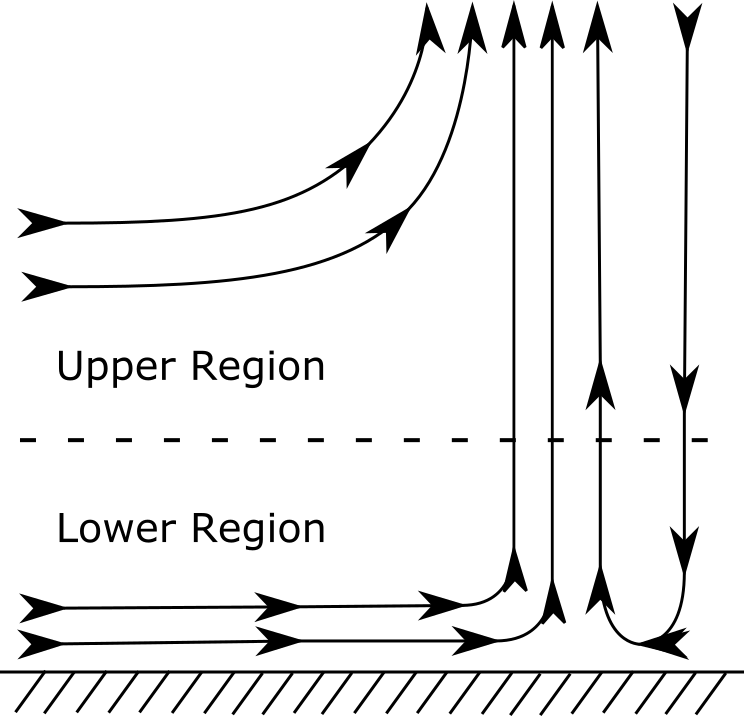
\includegraphics[width = 10 cm]{figs/ground}
     \caption{Cartoon of the structure of a dust devil. The lower region
     is the principle location of radial inflow, with the higher second
     layer flow becoming entrained by the upwardly circulating vortex. }
     \label{fig:cartoon}
    \end{center}
  \end{figure}


\subsection{Estimate of Energy Scaling}

Here we provide a rough estimate of the energy
available to a dust devil. There are two objectives behind this
analysis. The first is to provide justification for the concept of
extracting energy from these phenomena, with the reasoning that should
sufficient energy be available, then attempting to extract it might be
worthwhile. The second objective is to provide a simple analysis that
can serve as a measure of the efficiency of the generation process,
e.g. ``What fraction of the available energy are we extracting?''.  

At present, we consider only the energy flowing into the entrainment
region due to the ambient conditions, in particular, the incoming wind
and heat through the front hemisphere of a cylindrical region. We
consider a medium-sized (3m radius) dust devil with an incoming
freestream velocity of 5 m/s. The surface temperature is 343 Kelvin,
with a specified inflow boundary layer bridging the ground temperature
to the ambient air conditions of 313 Kelvin. 
% cite this?
\footnote{\normalsize These numbers were selected based on information
provided by the Georgia Tech field team in Arizona during the summer of
2014.} 

There are two forms of energy to consider: kinetic and gravitational
potential. First, we examine the kinetic energy flux through the front
of the apparatus. From the first law of thermodynamics we can express
the kinetic energy flux as a surface integral over the upstream face of
the device,  
\begin{equation*}
\text{KE} = \int_{CS} \frac{\vec V^2}{2} \rho \vec V \cdot \hat n dA.
\end{equation*}
%
% could cite fluid dynamics book here
% pg. 239
%
We make several simplifying assumptions. We assume our freestream 
velocity has no components in the span and height. 
We further assume that the variation in height for the streamwise
velocity is only on account of the thin boundary layer near the
ground. We functionally approximate this behavior using the common 7th
power function for a turbulent boundary layer,  
\begin{equation*}
  u(z) = U \text{ min }\left(\left(\frac{z}{\delta}\right)^7,1\right)
\end{equation*}
where U is the constant freestream velocity and $\delta$ the assumed
boundary layer thickness. Our integral can be solved to show, 
\begin{align*}
\text{KE} & = -R \rho U^3 \left[ z_{\text{max}} - \frac{10}{11}\delta.
\right]
\end{align*}

%%  & = \frac{1}{2} R \rho u^3 z_\text{max}
%%  \int^{\frac{3\pi}{2}}_{\frac{\pi}{2}} \text{cos}\theta d\theta \\
%%  & = -R \rho u^3 z_\text{max}. 
%% \end{align*}

The negative sign here indicates that the kinetic energy is flowing into
the surface, in opposition to the outward facing unit normal, $\hat
n$. Characteristic values for this analysis are, $u = 5$ m/s, $\rho =
1.225$ Kg/$m^3$, $R = 3$ m, and $z_{\text{max}} = 2.5$ m. The boundary
layer thickness is $\approx 10$ cm. This provides
an estimate of 1144.26 Watts as the incoming kinetic energy flux. Or,
approximately 1.14 kW.  

We estimate the gravitational potential
energy flux by integrating the boussinesq term by the height of the vanes, 
\begin{align*}
  \text{Potential Energy Flux} & = \int_{-h}^0 u(z) \Delta \rho g z dz. \\
  & = \int_{-h}^0 u(z) \rho' g z^2 dz. 
\end{align*}
Where the substitution, $\Delta \rho = \rho' z$ was made. We again
assume the boundary layer follows the 7th order profile, and 
% At 
% this point we again separate the integral into two components, 
% for the boundary layer and the constant freestream velocity region. 
% \begin{align*}
%   & = \rho' g \left[ \int_{-\delta}^{0} U \left( \frac{z}{\delta} \right)^7 z^2 dz 
%       + \int_{-h}^{-\delta} U z^2 dz \right] \\
%   & = -\rho' g U \left[ \frac{h^3}{3} - \frac{7}{30} \delta^3 \right].
% \end{align*}
% Furthermore, we note 
%
that $\rho' = -\beta \rho_0 \Delta T$, resulting in, 
%
% cite monin-yaglom page 59
%
\begin{equation}
 \text{Power } = U \beta \rho_0 \Delta T g \left[ \frac{h^3}{3} -
					    \frac{7}{30} \delta^3
					   \right]. 
\end{equation}

Using $\rho_0 = 1.225$ Kg/$m^3$, $T_{\text{ref}}=313$m Kelvin, $\beta_T
= 0.003194$ (This is just 1/$T_{\text{ref}}$), $g=9.81$ m/$s^2$, and a
freestream velocity of five meters per second results in an
estimate of 30 Watts for the gravitational potential energy. 

This interesting result implies that the majority of the available
energy is attributable to kinetic energy, not the gravitational
energy. 
% todo: think about renno
%This is inconsistent with the results of
%Renno\cite{}\todo{missing cite here}, who demonstrated
%that the available thermal energy present was not sufficient to account
%for the velocities measured in dust devils. 
However, while the
gravitational potential energy is a small fraction of the energy
available, that does not imply it is without significant impact. The
extent to which the thermal energy acts as an assisting mechanism for 
``lifting-up'' the flow is unclear, but given the observed increase in dust
devil formation during peak thermal gradients, it is expected
to play an important role. 

\subsection{Dust Devil Generation Concept}

The preceding discussion has justified the idea that 
dust devils are carriers of non-trivial levels ambient kinetic and
gravitational potential energy from the environment. This  
subsection now provides a brief discussion of how the physics of 
dust devils informs the generation of a synthetic variety, so that these
phenomena might be used as a means of extracting usable work. 

In contrast to the naturally occuring dust devils
our synthetic solar driven vortex, (SoV) design makes use of
control surfaces to dictate the angle of incoming flow, and in doing so
explicitly converts a portion of the incoming radial flow in azimuthal
velocity. These turning vanes also serve as an anchor for the synthetic
vortex, locking it into a small region. An abstract concept of the turning
vane geometry is shown in figure \ref{fig:cartoon_vanes}.

Our observations of the naturally occuring dust devils informs some of
our \textit{a priori} expectations for the design of the turning
vanes. The bottom tier are designed to reside in the lower region, where
the principle inflow will occur. We therefore expect a radial or nearly
radial start to the vanes, which becomes increasingly tangential as the
flow moves towards the center. The inner radius of the bottom tier will
correspond to the outer radius of the generated vortex. 

The top tier serves a different purpose. We expect a non-zero initial
angle, as this tier is also designed to protect the rising vortex from
being blow away by ambient winds. The vanes radius will be shorter, as
the flow from this tier becomes entrained and the vortex grows in
size. 

For both the upper and lower tiers, our objective is to strike a balance
between effectively turning the incoming flow to impart azimuthal
velocity, while simultaneously not introducing such a high angle that
the vanes act as a blocking surface which the incoming flow will move
around. For instance, when the inlet angles are too severe, the vanes
block the incoming flow, which results in an adverse pressure gradient
existing near the outside edge of the 
vanes. This serves to force fluid around and over the system, instead
of inside the turning vanes. This reduces the velocity of flow inside
the system, resulting in a weaker thermal vortex.  To reduce
the flow blockage, we use gently curving vanes. A gentler angle permits
more flow to enter the vane region, after which the curvature increases
toward the center of the vanes. In this way, the angle smoothly varies
between a nearly zero angle at the outside edge of the vanes to a
maximum angle at a specified inner radius.

  \begin{figure}[!htb]
    \begin{center}
     \includegraphics[width = 8 cm]{figs/ground_vanes}
     \caption{Image of a possible two tier turning vane 
       configuration for generating synthetic dust devils.}
     \label{fig:cartoon_vanes}
    \end{center}
  \end{figure}

%% \Begin{figure}[h]
%%  \begin{center}
%%   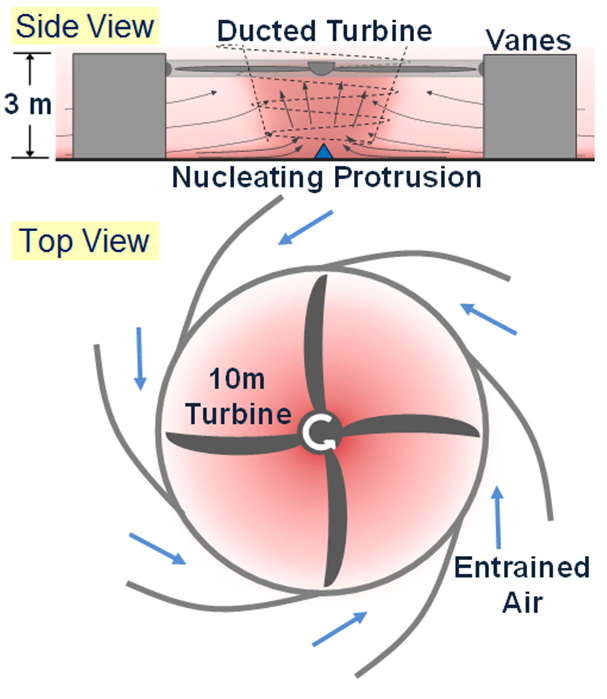
\includegraphics[width=.5\linewidth]{fig/power_generation.png}
%%    \caption{The Sov facility, showing the vanes, rotor and anchoring
%%    protrusion, as well as the buoyancy-driven vortex used to drive the
%%    turbine.}
%%    \label{facility}
%%   \end{center}
%% \end{figure}

Our principle objective is to use a synthetic dust devil to produce 
usable work. To extract the energy from the synthetic dust
devil, a turbine is placed 
at or near the top of the second tier of turning vanes. 
The blades of the turbine will be driven by the dust devil's azimuthal
and vertical velocities. While the Betz limit\cite{betz} gives a reasonable
expectation of the efficiency with which energy can be expected to be
extracted from the ambient dust devil velocity field, there are other
non-trivial design considerations. In particular, the impact of the
turbine on the dust devil's vortex, and any potential disruption of the
flow on account of the turbine must be investigated. Optimizing the
turbine to maximize the energy extraction while simultaneously
minimizing it's impact on the character of the dust devil's solution
will be an important issue.

While the turning vanes and turbine  
paradigm represents a reasonable starting point for design, the
parameter space of possible system configurations is large. It is
unclear how to engineer an effective SoV system. Important design
consideration include: 
\begin{itemize}
  \item How should the turning vanes be configured?
  \item How does the energy produced scale with system diameter?
  \item Are additional surfaces, such as a cone, capable of increasing energy output?
\end{itemize}

Questions such as these provide the principle impetus of using
computational fluid dynamics (CFD) to inform system design. The
parameter space of conceivable system designs is far larger than can be
probed experimentally, and even if such a campaign were to be embarked
upon, it would be at significantly greater temporal and monetary
cost. The subsequent chapter will provide the mathematical basis by which
we model the system, so that we can then begin to discuss how we might
optimize it computationally.  


